
\documentclass[12pt]{article}

% Layout.
\usepackage[top=1in, bottom=0.75in, left=1in, right=1in, headheight=1in, headsep=6pt]{geometry}

% Fonts.
\usepackage{mathptmx}
\usepackage[scaled=0.86]{helvet}
\renewcommand{\emph}[1]{\textsf{\textbf{#1}}}

% TiKZ.
\usepackage{tikz, pgfplots}
\usetikzlibrary{calc}
\pgfplotsset{compat = newest}
 
\pgfplotsset{my style/.append style={axis x line=middle, axis y line=
middle, xlabel={$x$}, ylabel={$y$}, axis equal }}

% Misc packages.
\usepackage{amsmath,amssymb,latexsym}
\usepackage{graphicx}
\usepackage{array}
\usepackage{xcolor}
\usepackage{multicol}

% Commands to set various header/footer components.
\makeatletter
\def\doctitle#1{\gdef\@doctitle{#1}}
\doctitle{Use {\tt\textbackslash doctitle\{MY LABEL\}}.}
\def\docdate#1{\gdef\@docdate{#1}}
\docdate{Use {\tt\textbackslash docdate\{MY DATE\}}.}
\def\doccourse#1{\gdef\@doccourse{#1}}
\let\@doccourse\@empty
\def\docscoring#1{\gdef\@docscoring{#1}}
\let\@docscoring\@empty
\def\docversion#1{\gdef\@docversion{#1}}
\let\@docversion\@empty
\makeatother

% Headers and footers layout.
\makeatletter
\usepackage{fancyhdr}
\pagestyle{fancy}
\fancyhf{} % Clears all headers/footers.
\lhead{\baselineskip 30pt
%\emph{\@doctitle\hfill\@docdate}
\emph{\@docdate\hfill\@doctitle}
\ifnum \value{page} > 1\relax\else\\
\emph{Name: \rule{3.5in}{1pt}\hfill \@docscoring}\fi}
\rfoot{\emph{\@docversion}}
\lfoot{\emph{\@doccourse}}
\cfoot{\emph{\thepage}}
\renewcommand{\headrulewidth}{0pt}%
\makeatother

% Paragraph spacing
\parindent 0pt
\parskip 6pt plus 1pt

% A problem is a section-like command. Use \problem{5} to
% start a problem worth 5 points.
\newcounter{probcount}
\newcounter{subprobcount}
\setcounter{probcount}{0}
\newcommand{\problem}[1]{%
\par
\addvspace{4pt}%
\setcounter{subprobcount}{0}%
\stepcounter{probcount}%
\makebox[0pt][r]{\emph{\arabic{probcount}.}\hskip1ex}\emph{[#1 points]}\hskip1ex}
\newcommand{\thesubproblem}{\emph{\alph{subprobcount}.}}

% Subproblems are an enumerate-like environment with a consistent
% numbering scheme. 
% Use \begin{subproblems}\item...\item...\end{subproblems}
\newenvironment{subproblems}{%
\begin{enumerate}%
\setcounter{enumi}{\value{subprobcount}}%
\renewcommand{\theenumi}{\emph{\alph{enumi}}}}%
{\setcounter{subprobcount}{\value{enumi}}\end{enumerate}}

% Blanks for answers in normal and math mode.
\newcommand{\blank}[1]{\rule{#1}{0.75pt}}
\newcommand{\mblank}[1]{\underline{\hspace{#1}}}
\def\emptybox(#1,#2){\framebox{\parbox[c][#2]{#1}{\rule{0pt}{0pt}}}}

% Misc.
\renewcommand{\d}{\displaystyle}
\newcommand{\ds}{\displaystyle}
\def\bc{\begin{center}}
\def\ec{\end{center}}
\def\be{\begin{enumerate}}
\def\ee{\end{enumerate}}


\doctitle{Math 251: Quiz 4}
\docdate{Feb 9, 2023}
\doccourse{UAF Calculus I}
\docversion{v-1}
\docscoring{\blank{0.8in} / 25}
\begin{document}
%\textbf{Please circle your instructor's name:} \hfill Leah Berman  \hfill   Jill Faudree\\

There are 25 points possible on this quiz. No aids (book, calculator, etc.)
are permitted.  {\bf Show all work for full credit.}

\begin{enumerate}
\item (8 points) \emph{Use the definition of the derivative} (provided below) to find the derivative of the function $\ds f(x)= \frac{2}{3x}.$ No credit will be awarded for finding the derivative via other methods.\\

$\ds f'(x)=\lim_{h \to 0} \frac{f(x+h) - f(x)}{h}$

\vfill

\item (4 points) The function $H(x)$ is graphed below. Sketch the graph of $H'(x),$ the derivative of $H(x)$, on the same set of axes.\\

\begin{center}
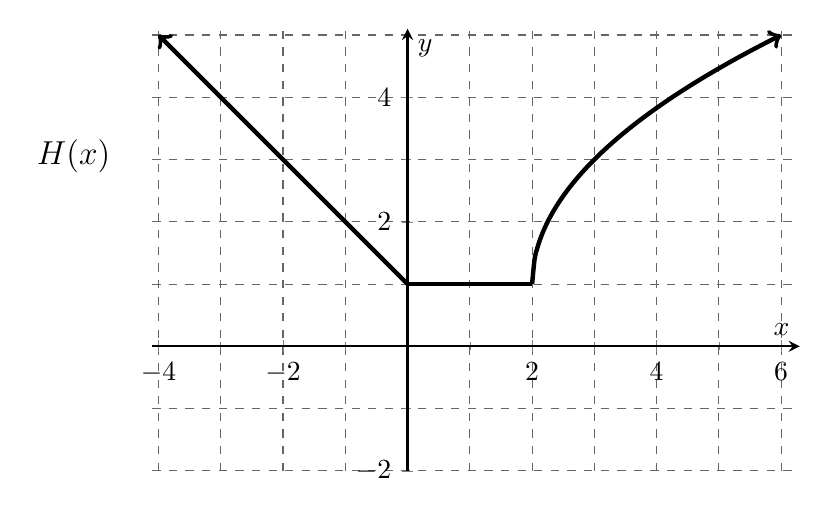
\begin{tikzpicture}
\begin{axis}[scale=1.2, thick, my style, xtick={-4,-2,...,6}, ytick={-2,0,2,...,6},
xmin=-4.1, xmax=6.3, ymin=-2, ymax=5.1, minor y tick num=1,
        minor x tick num=1, mark size=3.0pt, grid=both, grid style={ thin, black!60, dashed}, axis equal image]
%%Curves
%\addplot[<-,ultra thick, smooth, variable=\x, samples=100, domain=-4.8:-2] plot(\x,{1/(\x+5) - 0.333});
\addplot[ultra thick, smooth,<-] coordinates {(-4,5) (0,1)};
\addplot[ultra thick, smooth] coordinates {(0,1) (2,1)};
\addplot[->,ultra thick, smooth, variable=\x, samples=100, domain=2:6] plot(\x,{1+2*(\x-2)^(0.5)});    
\end{axis}
\node at (-1,4){\large{$H(x)$}};
\end{tikzpicture}
\end{center}

\newpage
\item (9 points) Find $f'(x)$ for each function below. You do not need to simplify your answer.
	\begin{enumerate}
	\item $f(x)=8x^3-2\sqrt{x}+\sqrt{3}$
	\vfill
	\item $f(x)=(x+1)\cos(x)$
	\vfill
	\item $f(x)=\frac{\sin(x)}{5x-4}$
	\vfill
	\end{enumerate}
\item (4 points) The function $F(t)$ models the temperature  in degrees Celsius of a cabin $t$ minutes after a wood stove has been lit. 
	\begin{enumerate}
	\item Interpret  $F(20)=5$ in the context of the problem.
	\vspace{.7in}
	\item Interpret $F'(20)=1$ in the context of the problem.
	\vspace{.7in}
	\end{enumerate}
\end{enumerate}
\end{document}